\RequirePackage{luatex85}
\documentclass[tikz]{standalone}
\begin{document}
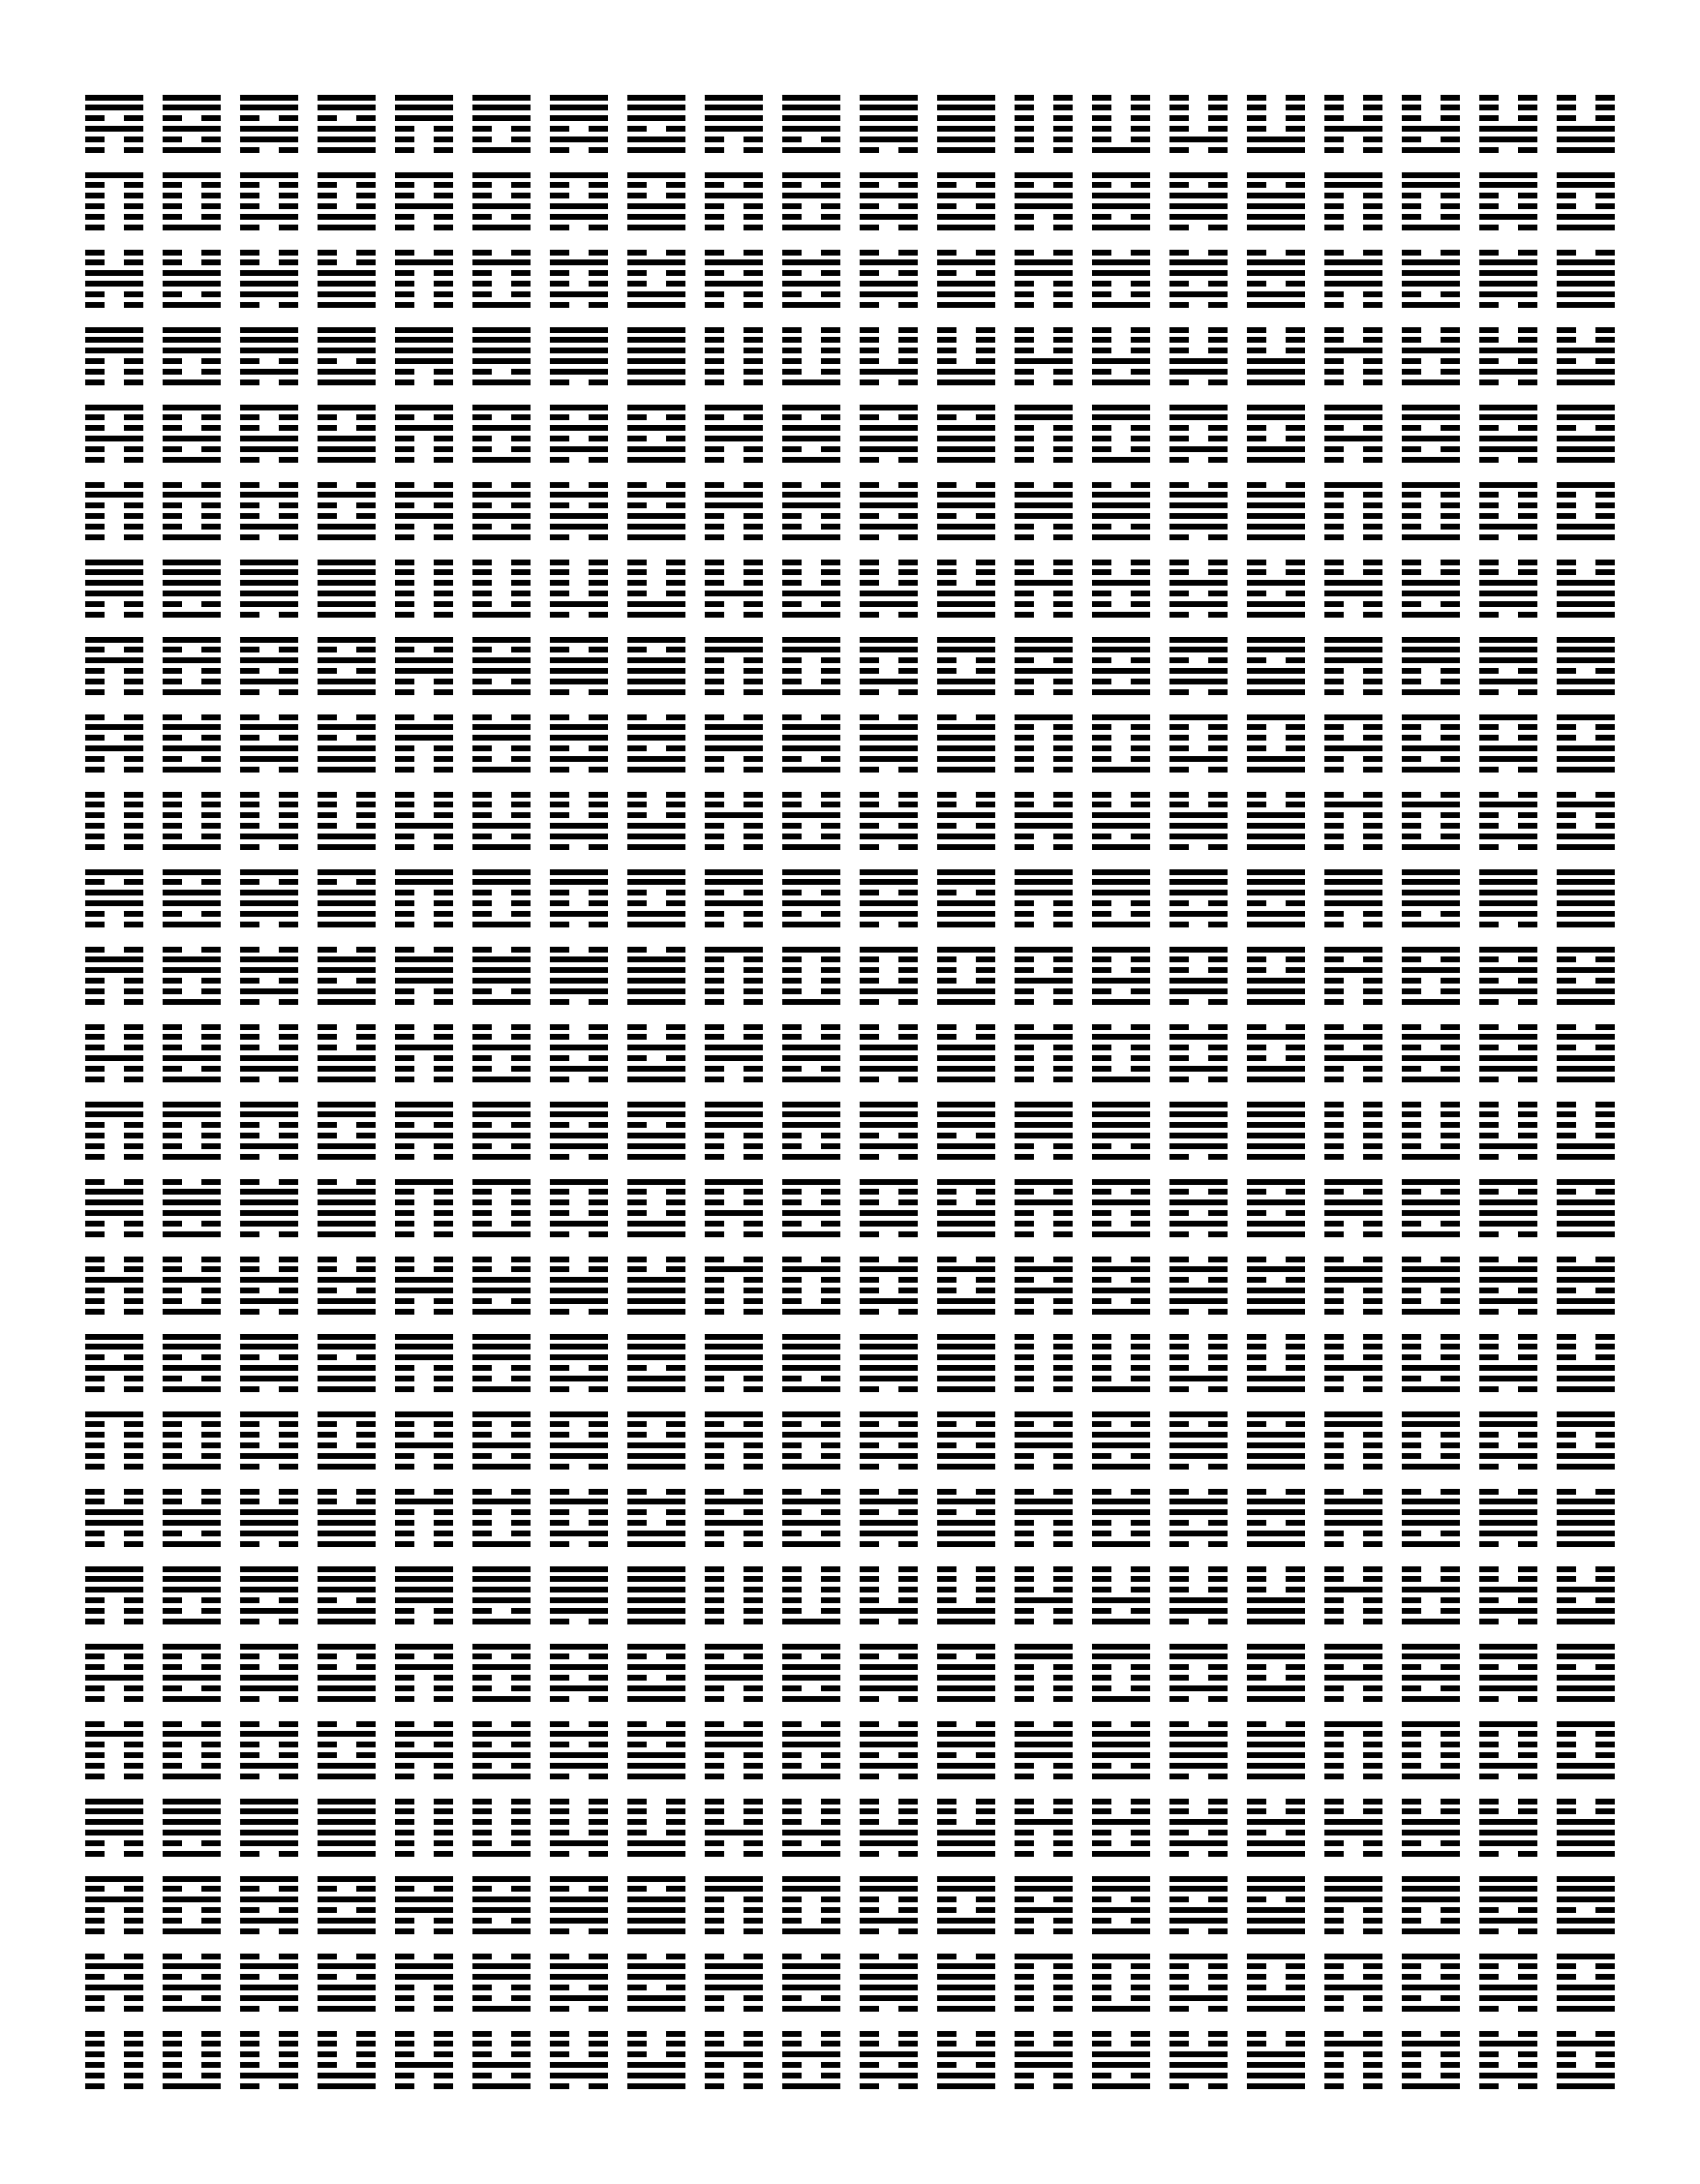
\begin{tikzpicture}
% 0.03in = \barwidth
[line width=0.03in]
\clip (0,0) rectangle (8.5in,11in);
\foreach \row in {0,...,25}{ % 25 = 26-1 = \numrows-1
\foreach \col in {0,...,19}{ % 19 = 20-1 = \numcols-1
\foreach \bar in {0,...,5}{
	% 0.3in = \leftmargin
	% 0.4in = 0.1in+0.3in = \xsep+\barlen
	% 0.365in = 0.35in+0.5*0.03in = \bottommargin+0.5*\barwidth
	% 0.054in = 0.03in+0.024in = \barwidth+\barsep
	% 0.4in = 6*0.03in+5*0.024in+0.1in = 6*\barwidth+5*\barsep+\ysep
	\draw ({0.3in+\col*0.4in}, {0.365in+\bar*0.054in+\row*0.4in}) coordinate (xy);
	% 20 = \numcols
	\pgfmathtruncatemacro\barval{mod(floor(mod(\col+20*\row,64)/2^\bar),2)}
	\ifnum\barval=0
	% 0.1in = \barlen/3
	% 0.3in = \barlen
	\draw (xy) -- ++(right:0.1in) ++(right:0.1in) -- ++(right:0.1in);
	\else\draw (xy) -- ++(right:0.3in);\fi
	}}}
%\draw[step=0.1in, thin] (0,0) grid (8.5in,11in);
\end{tikzpicture}

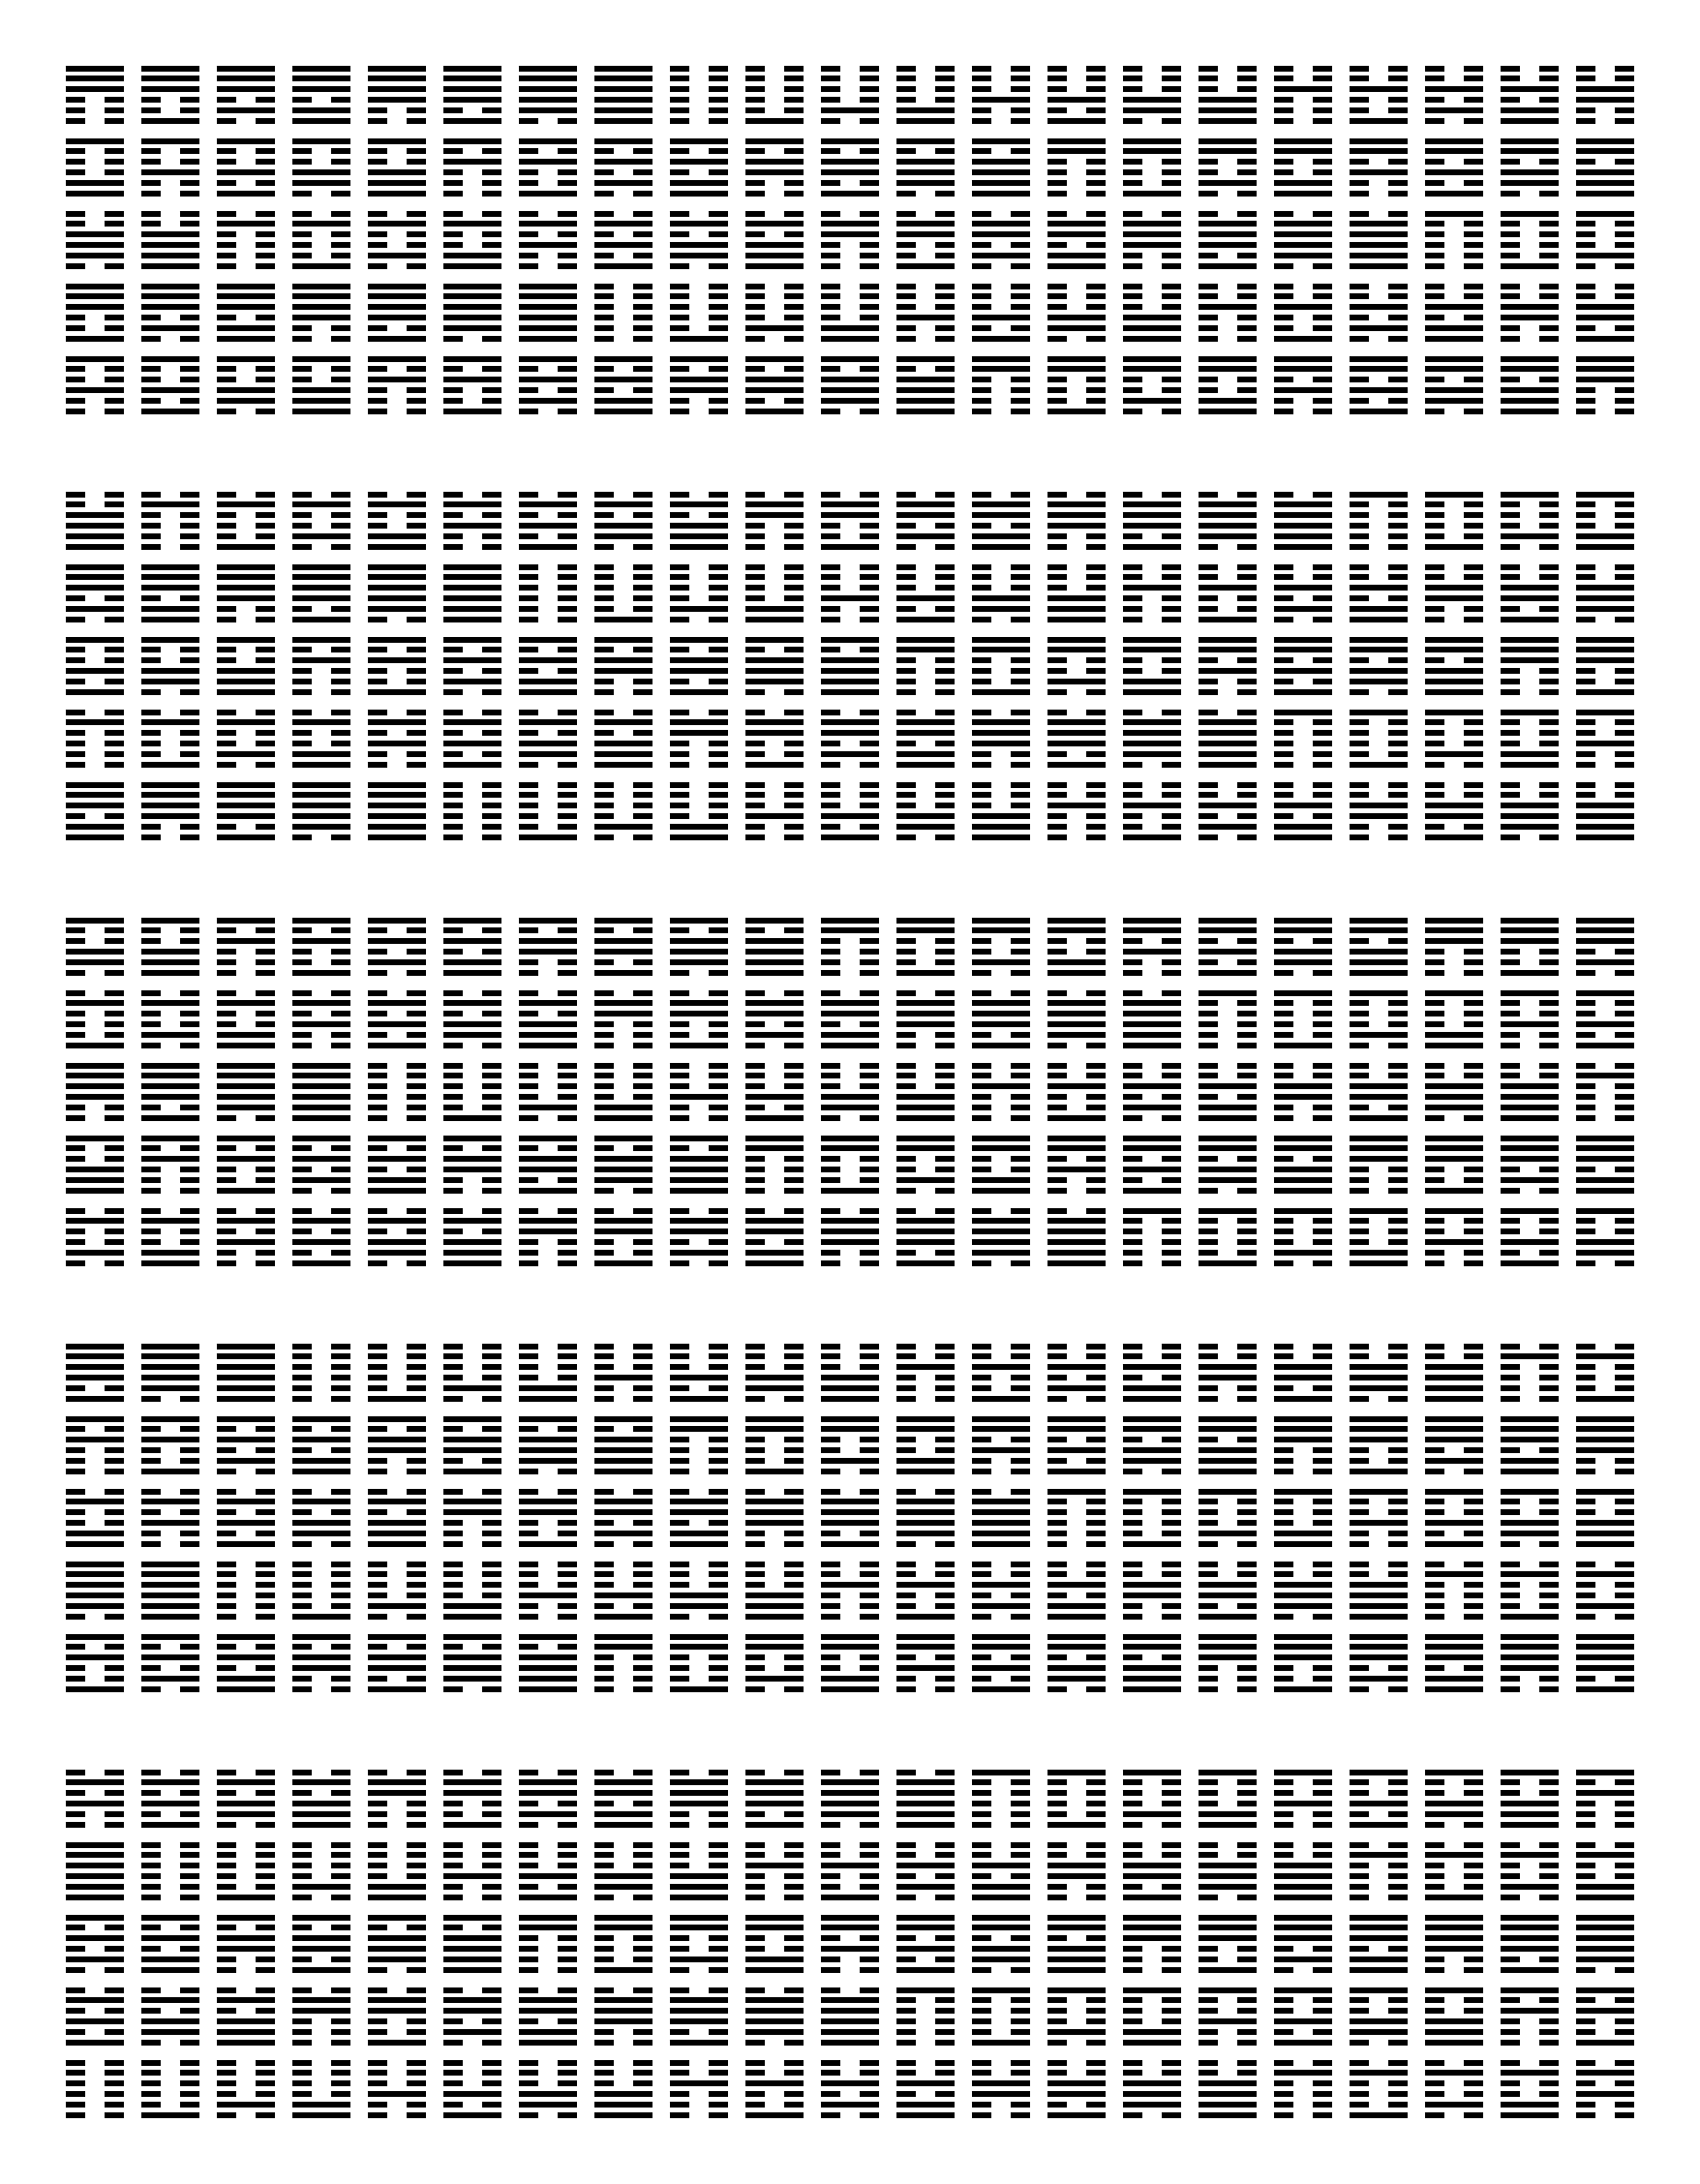
\begin{tikzpicture}
% 0.03in = \barwidth
[line width=0.03in]
\clip (0,0) rectangle (8.5in,11in);
\foreach \sec in {0,...,4}{ % 4 = 5-1 = \numsecs-1 
\foreach \row in {0,...,4}{ % 4 = 5-1 = \numrows-1
\foreach \col in {0,...,20}{ % 20 = 21-1 = \numcols-1
\foreach \bar in {0,...,5}{
	% 0.2in = \leftmargin
	% 0.39in = 0.09in+0.3in = \xsep+\barlen
	% 0.215in = 0.2in+0.5*0.03in = \bottommargin+0.5*\barwidth
	% 0.054in = 0.03in+0.024in = \barwidth+\barsep
	% 0.375in = 6*0.03in+5*0.024in+0.075in = 6*\barwidth+5*\barsep+\ysep
	% 2.2in = 11in/5 = 11in/\numsecs
	\draw ({0.2in+\col*0.39in}, {0.215in+\bar*0.054in+\row*0.375in+\sec*2.2in}) coordinate (xy);
	% 21 = \numcols
	% 105 = 21*5 = \numcols*\numrows
	\pgfmathtruncatemacro\barval{mod(floor(mod(\col+21*\row+105*\sec,64)/2^\bar),2)}
	\ifnum\barval=0
	% 0.1in = \barlen/3
	% 0.3in = \barlen
	\draw (xy) -- ++(right:0.1in) ++(right:0.1in) -- ++(right:0.1in);
	\else\draw (xy) -- ++(right:0.3in);\fi
	}}}}
%\draw[step=0.1in, thin] (0,0) grid (8.5in,11in);
\end{tikzpicture}

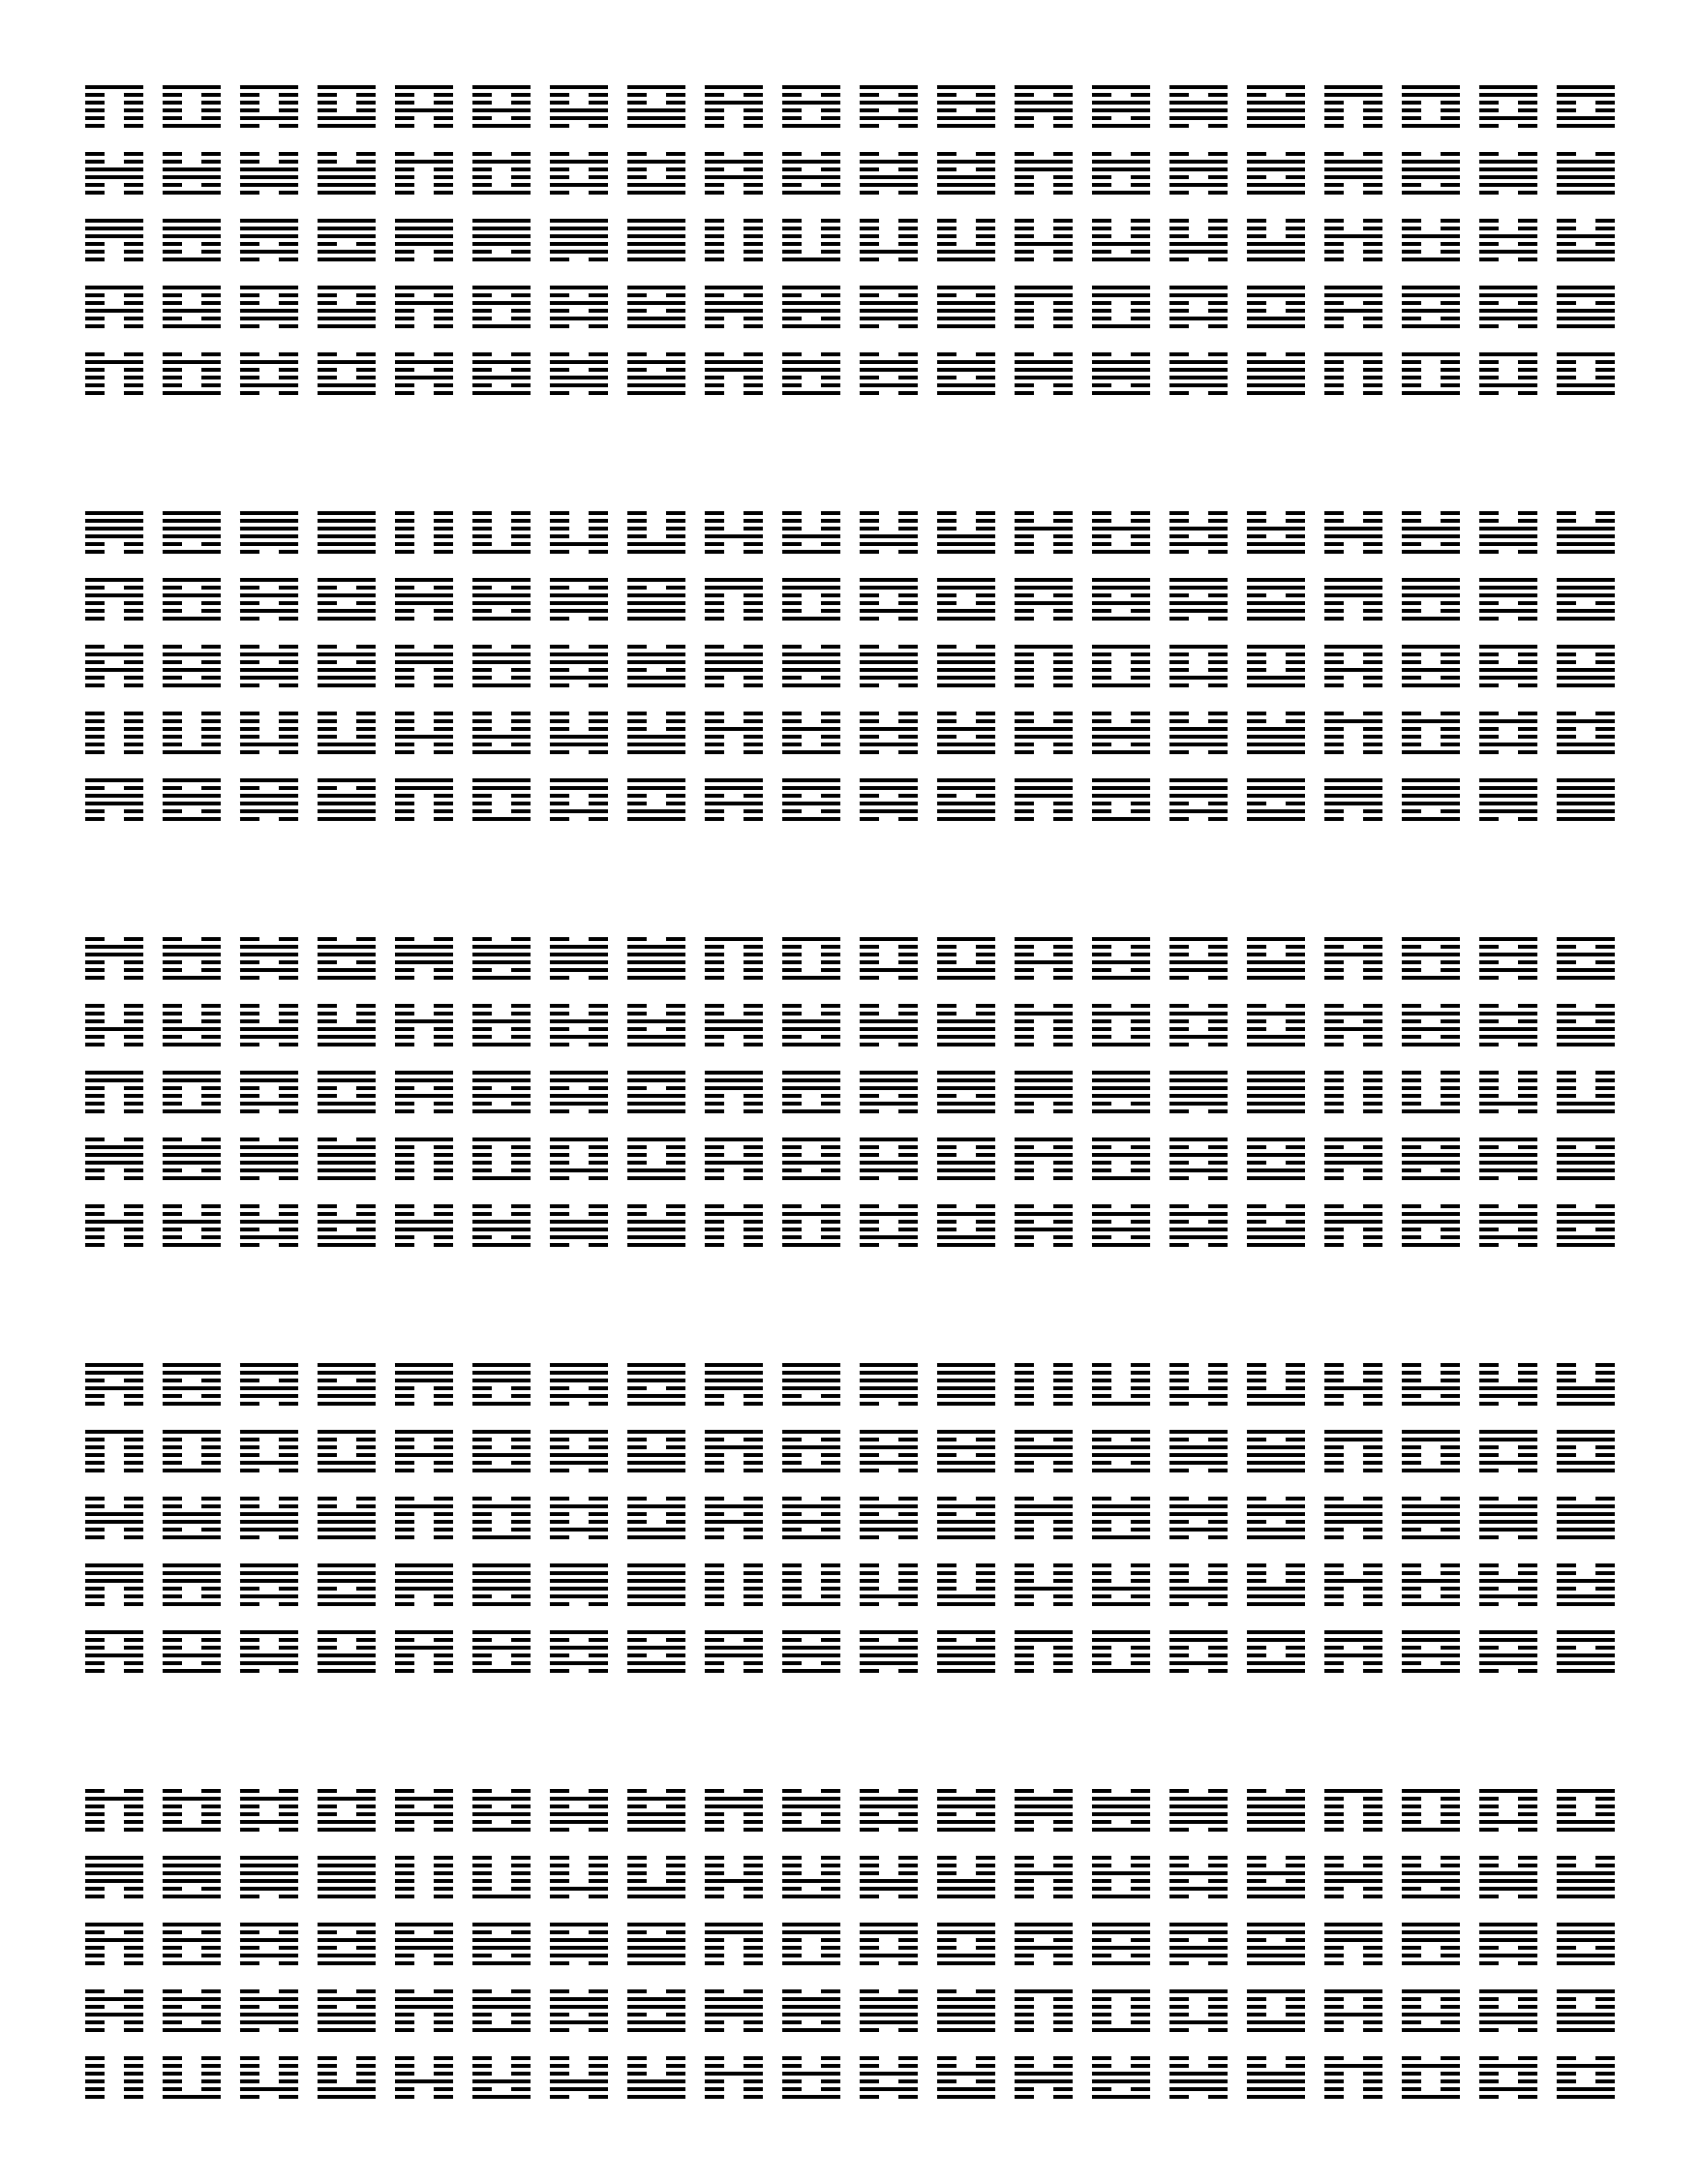
\begin{tikzpicture}
% 0.02in = \barwidth
[line width=0.02in]
\clip (0,0) rectangle (8.5in,11in);
\foreach \sec in {0,...,4}{ % 4 = 5-1 = \numsecs-1 
\foreach \row in {0,...,4}{ % 4 = 5-1 = \numrows-1
\foreach \col in {0,...,19}{ % 19 = 20-1 = \numcols-1
\foreach \bar in {0,...,5}{
	% 0.3in = \leftmargin
	% 0.4in = 0.1in+0.3in = \xsep+\barlen
	% 0.31in = 0.3in+0.5*0.02in = \bottommargin+0.5*\barwidth
	% 0.04in = 0.02in+0.02in = \barwidth+\barsep
	% 0.345in = 6*0.02in+5*0.02in+0.125in = 6*\barwidth+5*\barsep+\ysep
	% 2.2in = 11in/5 = 11in/\numsecs
	\draw ({0.3in+\col*0.4in}, {0.31in+\bar*0.04in+\row*0.345in+\sec*2.2in}) coordinate (xy);
	% 20 = \numcols
	% 100 = 20*5 = \numcols*\numrows
	\pgfmathtruncatemacro\barval{mod(floor(mod(\col+20*\row+100*\sec,64)/2^\bar),2)}
	\ifnum\barval=0
	% 0.1in = \barlen/3
	% 0.3in = \barlen
	\draw (xy) -- ++(right:0.1in) ++(right:0.1in) -- ++(right:0.1in);
	\else\draw (xy) -- ++(right:0.3in);\fi
	}}}}
%\draw[step=0.1in, thin] (0,0) grid (8.5in,11in);
\end{tikzpicture}

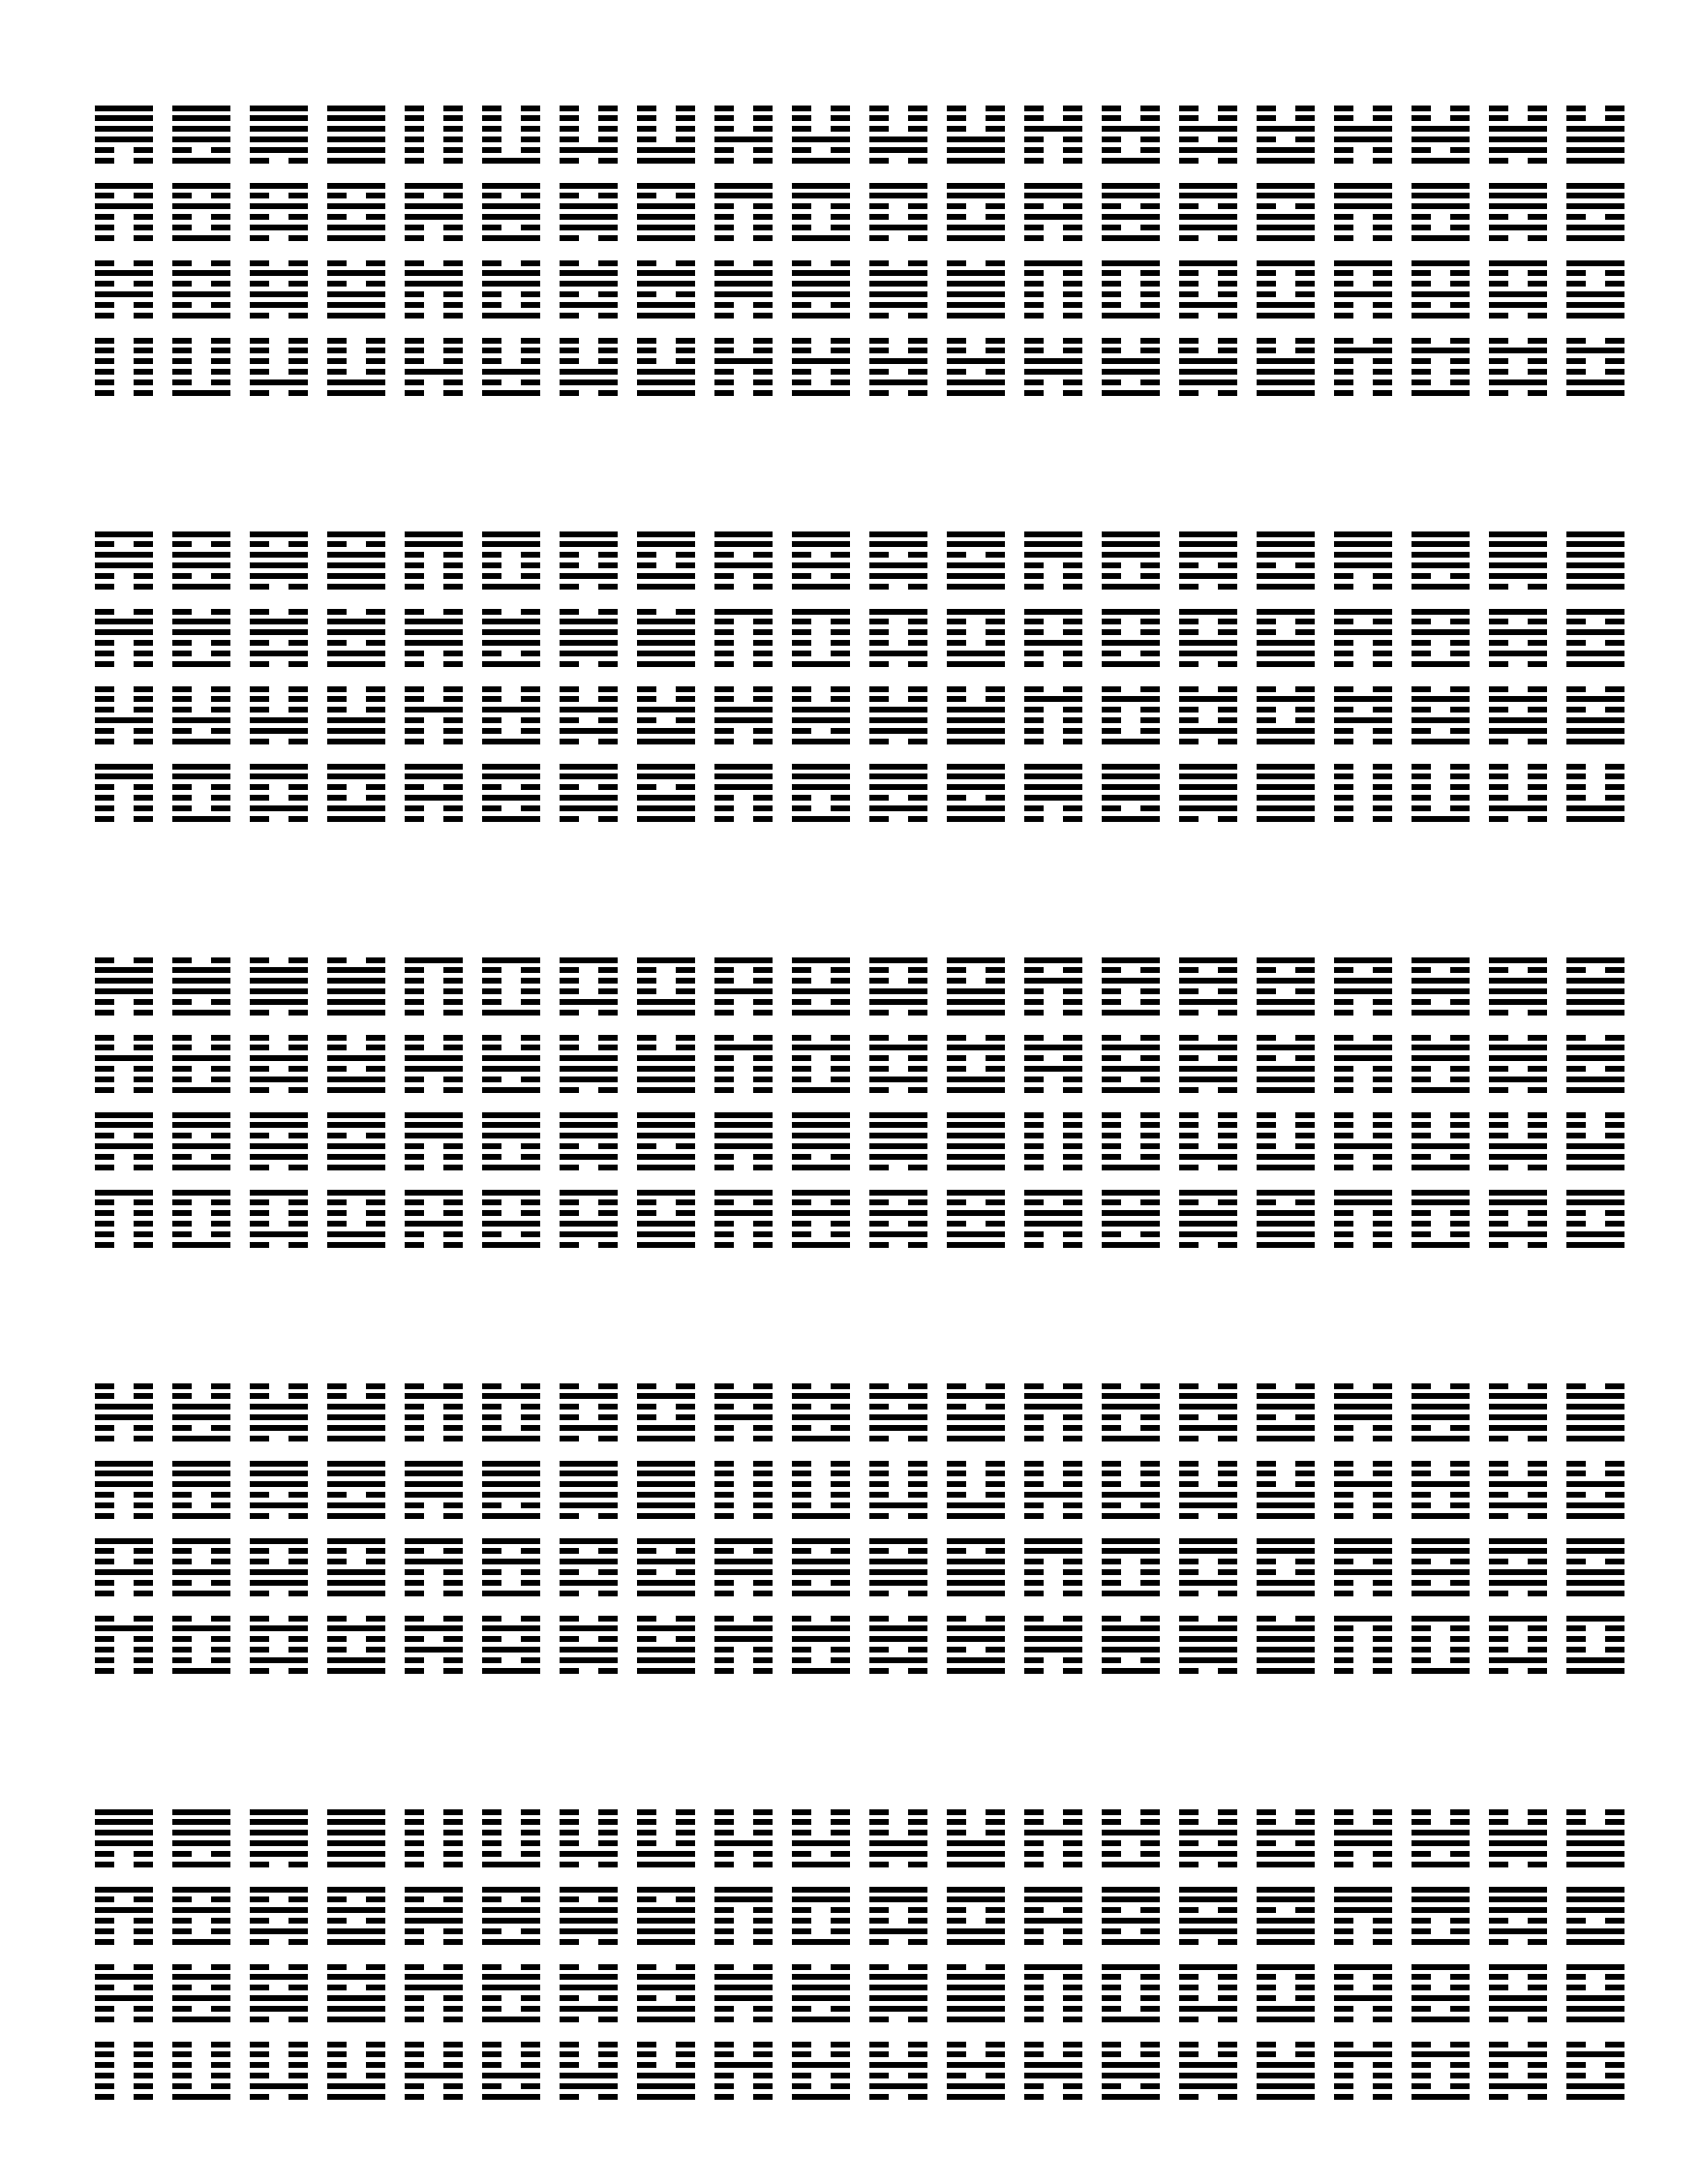
\begin{tikzpicture}
% 0.03in = \barwidth
[line width=0.03in]
\clip (0,0) rectangle (8.5in,11in);
\foreach \sec in {0,...,4}{ % 4 = 5-1 = \numsecs-1 
\foreach \row in {0,...,3}{ % 3 = 4-1 = \numrows-1
\foreach \col in {0,...,19}{ % 19 = 20-1 = \numcols-1
\foreach \bar in {0,...,5}{
	% 0.35in = \leftmargin
	% 0.4in = 0.1in+0.3in = \xsep+\barlen
	% 0.31in = 0.3in+0.5*0.02in = \bottommargin+0.5*\barwidth
	% 0.054in = 0.03in+0.024in = \barwidth+\barsep
	% 0.4in = 6*0.03in+5*0.024in+0.1in = 6*\barwidth+5*\barsep+\ysep
	% 2.2in = 11in/5 = 11in/\numsecs
	\draw ({0.35in+\col*0.4in}, {0.31in+\bar*0.054in+\row*0.4in+\sec*2.2in}) coordinate (xy);
	% 20 = \numcols
	% 80 = 20*4 = \numcols*\numrows
	\pgfmathtruncatemacro\barval{mod(floor(mod(\col+20*\row+80*\sec,64)/2^\bar),2)}
	\ifnum\barval=0
	% 0.1in = \barlen/3
	% 0.3in = \barlen
	\draw (xy) -- ++(right:0.1in) ++(right:0.1in) -- ++(right:0.1in);
	\else\draw (xy) -- ++(right:0.3in);\fi
	}}}}
%\draw[step=0.1in, thin] (0,0) grid (8.5in,11in);
\end{tikzpicture}
\end{document}